\chapter{Statistics-based Features}
\label{sec:statisticsfeatures}

Statistics-based temporal features are the first and most simplified category of temporal features developed. The main classes of features are basic temporal statistics, ratio-based, and the Spearman rank order correlation coefficient.

\section{Theoretical Basis}
\subsection{Basic Temporal Statistics}
\label{sec:basicstatistics}

The first set of temporal features to be extracted are basic statistics-based metrics that utilize the time-series data vector for various time ranges to obtain information using mean, median, maximum, minimum, range, variance, and standard deviation. Many of these features are developed through the implementation of the VISDOM package in the R programming language \citep{visdom_borgeson}.As a simple example, if a time-series vector is described as $X$, with $N$ values of $X = {x_1, x_2,...,x_n}$, the most common statistical metric, mean (or $\mu$), can be calculated using Equation \ref{eq:mean} \citep{Mitsa_2010}.

\begin{equation}
\mu = \frac{\sum\limits_{i=1}^N x_i}{N}
\label{eq:mean}
\end{equation}

The mean is taken not just for the entire time series, but also from the summer and winter seasons. The variance of the values are taken for the whole year, the summer and winter seasons as well. The variance of daily mean, minimum, and maximum values are determined to understand the breadth of values across the time range. Variance is calculated according to Equation \ref{eq:variance}. 


\begin{equation}
\sigma^2 = \frac{\displaystyle\sum_{i=1}^{n}(x_i - \mu)^2} {n}
\label{eq:variance}
\end{equation}

The maximum and minimum electrical demand are calculated. Additionally, the hour and date at which the maximum demand occurs are determined to understand when peak consumption occurs. Additionally, the temperature at the maximum and minimum is account for weather influence. The 97th and 3rd percentiles are calculated to exclude any extreme outliers, a value that's often more useful than the maximum and minimum.\\ 

A series of hour-of-day (HOD) metrics are calculated that relate to aggregating the behavior occurring at each of hour the day-four metrics. The first of these calculates the most current hour of the top demand of the top 10\% hottest days and the most common hour of the top 10\% temperatures to inform roughly about cooling energy consumption. These metrics are repeated from the bottom 10\% coldest days and temperatures. Another set of twenty-four metrics is calculated to account simply for the mean demand of each hour of the day.\\

A set of metrics is calculated individually for January and August to account for potential heating and cooling seasons. The daily maximum, minimum, mean, range and load duration are calculated for these seasonal periods. The complete list of these features can be found in Appendix \ref{sec:temporalfeaturelist}.


\subsection{Ratio-based Statistical Features}
\label{sec:ratiobasedfeatures}

%to get a sense of what a temporal feature is in the context of electrical meters for buildings, t

The second major category of statistical features is ratio-based features. Simply, these are metrics in which two or more of the previously calculated statistical metrics are combined as a ratio. These features often have a \emph{normalizing effect} in which buildings can be more appropriately compared to each other. The first extracted metric of this type is one of the most commonly calculated for building performance analysis: the consumption magnitude of electricity normalized by the floor area of the building. This metric seeks to provide a basis for comparison between buildings and is used as a key metric within numerous benchmarking and performance analysis techniques. Figure \ref{fig:normalizedmag} illustrates a single building example of this metric per hour across a time range of two weeks at the end of the year. The top line chart of this figure shows the magnitude of hourly electrical consumption for one of the case study buildings. The middle portion of the figure repeats this information in the form of a color-based, one-dimensional heatmap. In this example, the daily weekday profiles manifest themselves as light-colored bands and weekend and unoccupied periods as darker bands. The color bar at the bottom of the figure is key in interpreting the color values. This figure is an example of a single building demonstration of this particular feature and is a type of graphic that is used throughout this entire section.

\begin{figure}[ht!]
\begin{center}
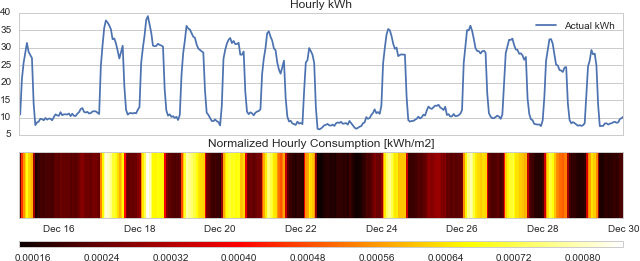
\includegraphics[width=1\columnwidth]{figures/normalizedcons_example/normalizedcons_example}
\caption{Single building example of area normalized magnitude
\label{fig:normalizedmag}%
}
\end{center}
\end{figure}

%  If a time-series vector is described as $X$, with $N$ values of $X = {x_1, x_2,...,x_n}$, the most common statistical metric, mean (or $\mu$), can be calculated using Equation \ref{eq:mean} \citep{Mitsa_2010}.

% \begin{equation}
% \mu = \frac{\sum\limits_{i=1}^N x_i}{N}
% \label{eq:mean}
% \end{equation}

After normalized consumption, the first set of temporal features to be extracted are primary statistics-based metrics that utilize the time-series data vector for various time ranges to retrieve information using mean, median, maximum, minimum, range, variance, and standard deviation. The median value of a vector is simply the middle value in an ordered set if the number of values is odd. If the length of the vector is even, then the median is the mean of the two middle values. The minimum and maximum values are the first and last in an ordered set. Vectors of values can also be described according to percentiles. Percentiles are cutpoints dividing the range of a probability distribution based on the percentage of values below a given threshold. For example, the value at the 95\% percentile is found 95\% of the way along an ordered set, with only 5\% of the values remaining before reaching the maximum. In this section, aggregation ratios of many of these collection techniques are applied to the 24 hours from a single day to characterize various types of typical behavior quickly. The first example of these ratios is the minimum versus maximum ratio or load ratio. This rate is calculated by taking the daily minimum and dividing it by the daily maximum. Figure \ref{fig:loadratio_singlebuilding} illustrates a single building example of this ratio on one month of data from a case study building. These load ratios indicated whether a daily profile is more diverse, resulting in a lower load ratio, or more flat, resulting in a higher load ratio. In this example, weekends and holidays are a darker shade of blue as compared to generally-occupied weekdays. Load ratio can be used an indicator also of the relative magnitude of the unoccupied baseline. Buildings that have a lower average load ratio often have higher than average baselines, such as in laboratories or hospitals.

\begin{figure}[ht!]
\begin{center}
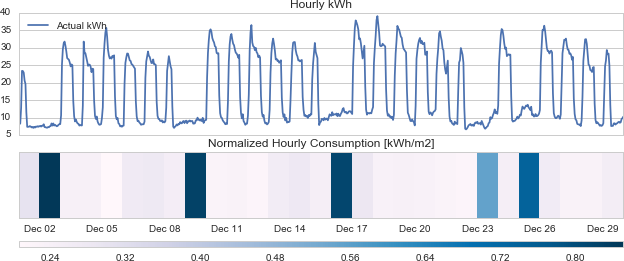
\includegraphics[width=1\columnwidth]{figures/loadratio_example/loadratio_example}
\caption{Single building example of the daily load ratio statistic
\label{fig:loadratio_singlebuilding}%
}
\end{center}
\end{figure}

% Daily load ratio is another simplified example of characterizing the minimum vs. maximum for each day.

% One of the primary functions of the built environment is to provide a thermally comfortable environment for occupants. These systems utilize electricity for the primary or secondary heating, ventilation, and air-conditioning systems (HVAC). Various metrics are developed in this effort to quantify the impact outdoor air conditions have on electricity performance.

A library of similar load ratio daily metrics is designed and implemented on the case study buildings. These other ratios are daily mean versus maximum, minimum versus 95\% percentile, and mean versus 95\% percentile. The use of the 95\% metric is mean to mitigate against outliers skewing the load ratios. These ratios are calculated on all days in the set, as well as just for weekend and weekdays. A full list of the features generated is found in Appendix A.

\subsection{Spearman Rank Order Correlation Coefficient}
\label{sec:weathercorrelationcoeff}

Data stream influence characterization is the process of roughly classifying the dataset into streams and subsequences based on weather conditions sensitivity. A feature is developed in a study of evaluation of campus data for simulation feedback, and the following is a summarization of this technique \citep{miller_forensically_2015}. This evaluation is important in understanding what measured performance is due to heating, cooling, and ventilation systems (HVAC) responses to outdoor conditions and what is due to schedule, occupancy, lighting, and different loading conditions which are weather independent. Performance data that is influenced by weather can be used to understand the HVAC system operation better or be weather-normalized to understand occupant diversity schedules. %Non-weather sensitive data streams are used with less pre-processing to create diversity schedules and to calculate miscellaneous and lighting load power densities. T

The Spearman Rank Order Correlation (ROC) is used to evaluate the positive or negative correlation between each performance measurement stream and the outdoor air dry bulb temperature. This technique has been previously used for weather sensitivity analysis \citep{coughlin_statistical_2009}. The ROC coefficient, $\rho$, is calculated according to a comparison of two data streams, $X$, and $Y$, in which the values at each time step, $X_i$, and $Y_i$, are converted to a relative rank of magnitude, $x_i$ and $y_i$, according to its respective dataset. These rankings are then used to calculate $\rho$ that varies between +1 and -1 with each extreme corresponding to a perfect positive and negative correlation respectively. A value of 0 signifies no relationship between the datasets. This $\rho$ value for a time-series is calculated according to Equation \ref{eq:spearman}.

\begin{equation}
\rho = 1 - \frac{6\sum d_i^2}{n(n^2-1)}
\label{eq:spearman}
\end{equation}

The difference between the data stream rankings, $x_i$ and $y_i$, is signified by a difference value, $d_i$, and the number of samples compared to each dataset is signified by $n$. Figure \ref{fig:weather_examples_plot} illustrates the calculation of the ROC coefficient, $\rho$ for three examples. The cooling sensitive data set shows a strong positive correlation between outside air temperature and energy consumption with a $\rho$ value of 0.934. As the outside air temperature increases, the power consumption measured by this meter increases. The heating sensitive dataset shown has a strong negative correlation with a $\rho$ of -0.68. A weather-insensitive dataset is shown in the middle which has a $\rho$ of 0.0, signifying no weather relationship, which is evident due to the four levels of consumption which are independent of outdoor air conditions.

\begin{figure}[ht!]
\begin{center}
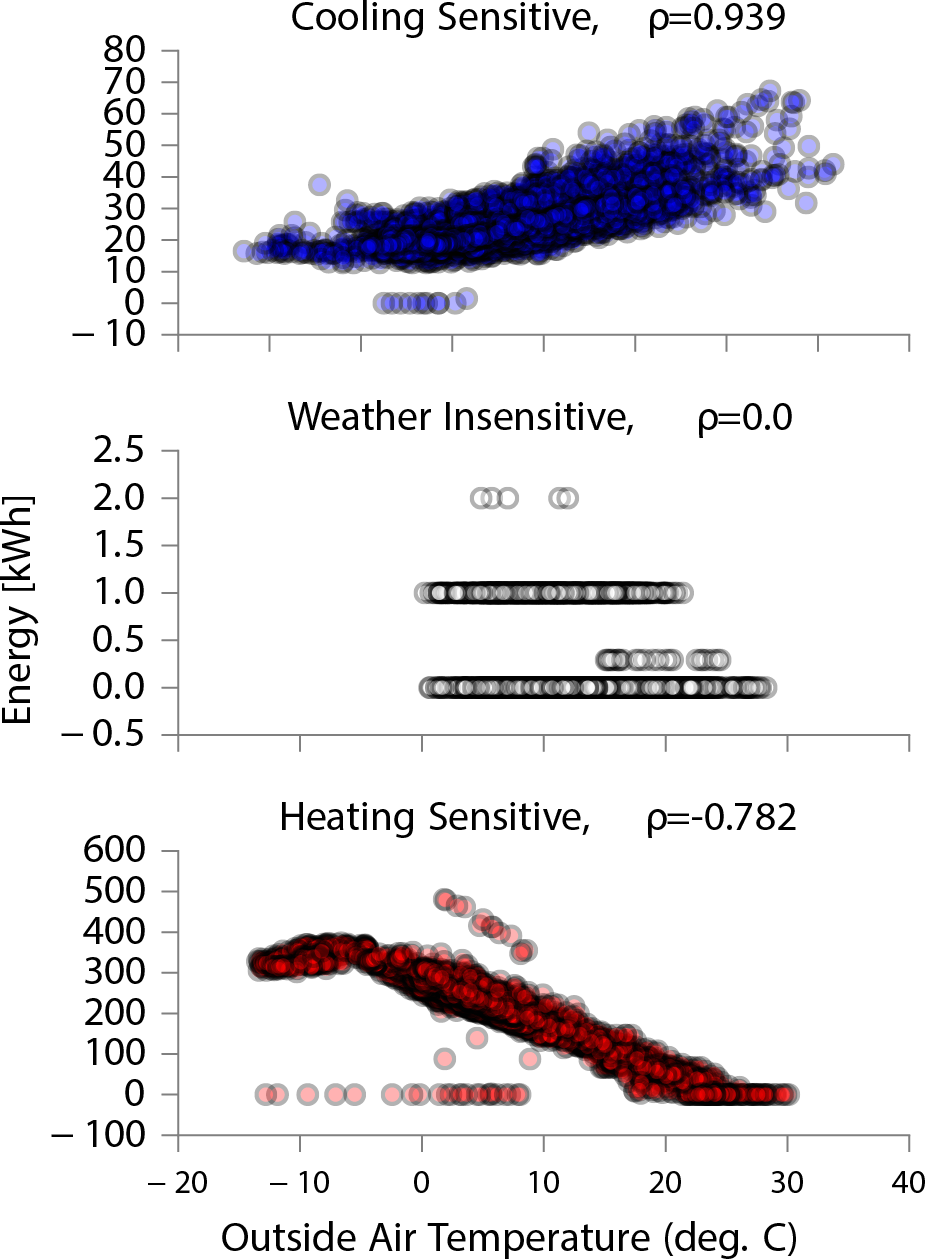
\includegraphics[width=0.5599999999999999\columnwidth]{figures/weathersensitivity/weathersensitivity}
\caption{Weather sensitivity examples as energy vs. outdoor air temperature (from \citep{miller_forensically_2015})
\label{fig:weather_examples_plot}%
}
\end{center}
\end{figure}

The correlation coefficient can be visualized for a single case as seen in Figure \ref{fig:spearman_singlebuilding}. The coefficient, in this case, is calculated individually for each month. This process results in twelve calculations of the metric using between 29-31 samples. In this case, consumption in January to May is noticeably more heating sensitive, a fact that can be observed clearly from the line chart, as well as the one dimension heat map. May to November is more cooling sensitive. It is interesting that September appears to be the most cooling sensitive month, a fact perhaps related to use schedules during that month. This coefficient is not a perfect indicator of HVAC consumption; it just detects a correlation. However, it is fast and easy to calculate and is the first phase of detecting weather dependency. More detailed and informative weather influence extraction features are investigated in Section \ref{sec:regressionmodels}.

\begin{figure}[ht!]
\begin{center}
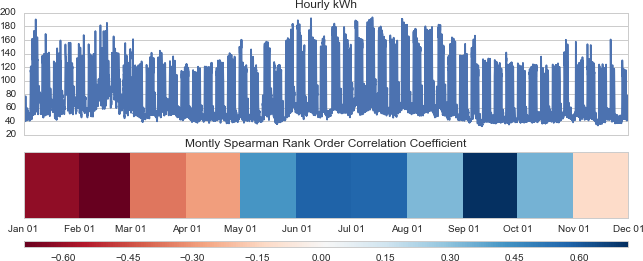
\includegraphics[width=1\columnwidth]{figures/spearman_example/spearman_example}
\caption{Single building example of the spearman rank order correlation coefficent with weather
\label{fig:spearman_singlebuilding}%
}
\end{center}
\end{figure}

\section{Implementation and Discussion}
Figure \ref{fig:normalizedcons_heatmap} illustrates the same normalized consumption metric as applied to all of the case study buildings. There are five segments of buildings based on the primary use types within the set: offices, university laboratories, university classrooms, primary/secondary schools, and university dormitories. These metrics are visualized in this way to understand the difference between each of these use types for each of the presented metrics. Each row of the heatmap for each segment is the values of the feature for a single building, while the x-axis is the time range for all buildings. Not all of the case study buildings have a January to December time range. For these cases, the data was rearranged so that a continuous set of January to December data is available to be visualized in the heat map. The aggregation metrics themselves are not calculated with this rearranged vector; it is only for visualization purposes. Like Figure \ref{fig:normalizedmag}, this type of graphic is used to visualize many of the temporal features in this section. From this metric in particular, one will notice that university labs have a systematically higher consumption over time as compared to the other use types. One will also see the dark vertical lines across the time range indicating weekend use as compared to the weekday. This particular pattern is absent from university dormitories due to their more continuous energy consumption.

\begin{figure}[ht!]
\begin{center}
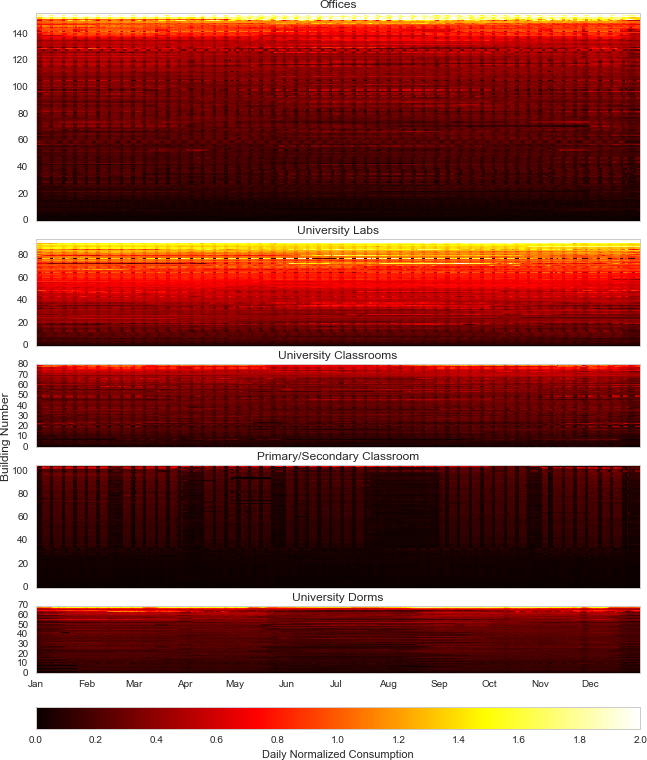
\includegraphics[width=1\columnwidth]{figures/normalizedcons_heatmap/normalizedcons_heatmap}
\caption{Heat map representation of normalized magnitude
\label{fig:normalizedcons_heatmap}%
}
\end{center}
\end{figure}

Figure \ref{fig:loadratio_heatmap} illustrates this metric as applied to all case study buildings. As in the normalized magnitude, various patterns are more apparent including the weekday versus weekend phenomenon.

\begin{figure}[ht!]
\begin{center}
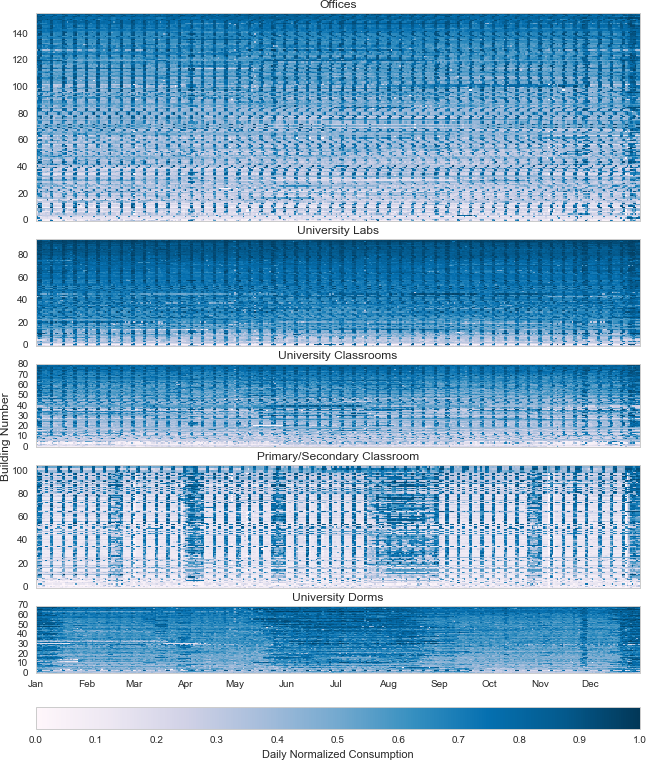
\includegraphics[width=1\columnwidth]{figures/loadratio_heatmap/loadratio_heatmap}
\caption{Heatmap of daily load ratio statistic for all case study buildings
\label{fig:loadratio_heatmap}%
}
\end{center}
\end{figure}

\begin{figure}[ht!]
\begin{center}
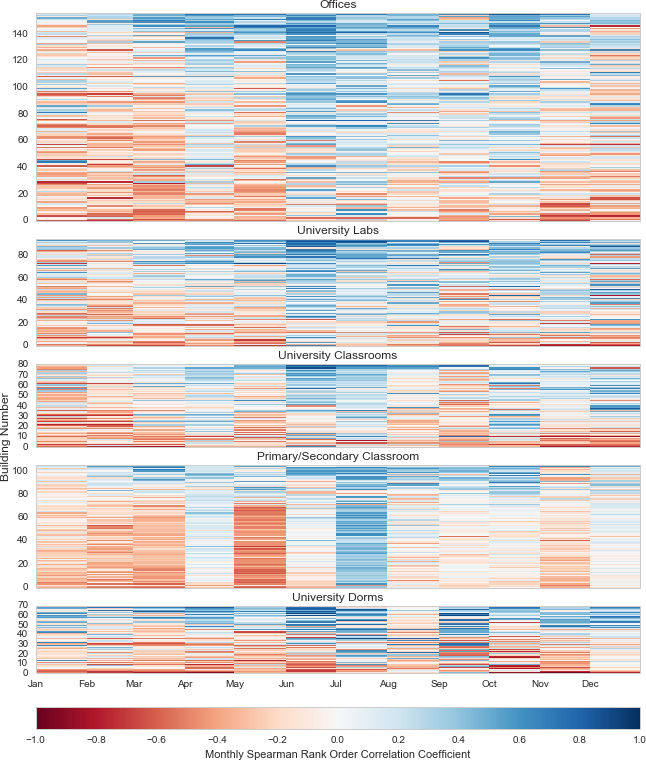
\includegraphics[width=1\columnwidth]{figures/spearman_heatmap/spearman_heatmap}
\caption{Heatmap of spearman rank order correlation coefficient for all case study buildings
\label{fig:spearman_heatmap}%
}
\end{center}
\end{figure}

